\chapter{Introduction}
\label{chap/intro} 

Three dimensional object recognition is a fundamental problem in computer vision. It spans the various topics of detection, identification, classification and pose estimation of 3D objects in spatial and spatiotemporal visual data, including point clouds, depth image sequences,volumetric scans and videos.

% Add a new paragraph for potential applications?  

The topics of 3D object recognition have been studied extensively since the early days of computer vision research. 
% Pioneer articulated very different framework for representing and recognising 3D objects. 
Pioneers of computer vision have proposed various models for representing and recognising objects from different types of 3D visual data.
% The number of literature reflected how the early researher treat the topic seriously. 
% Marr 
For instance, in late 1970s, Marr and Nishihara \cite{Marr1978} presented the primal sketch, in which a 3D shape is represented as a hierarchical set of cylinders positioned in an object-centric frame. 
% Generalised cone by Nevatia 
Meanwhile, Nevatia and Binford \cite{Nevatia1977} proposed the generalised cones framework to describe and recognise 3D geometric shapes. Bolles \etal \cite{Bolles1983} studied the pose estimation of 3D shapes from depth maps.  
% Moving light display
Concerning 3D object recognition in spatiotemporal data, human actions is regarded as a common target, which is widely available in video data. The study of action classification was emerged around the same time with computer vision research in the 1970s. For example, Johansson \cite{Johansson1973} pioneered video-based action recognition using a moving light display. However, articulated pose estimation of human actions had not been studied until almost a decade later in early 1980s, \eg Hogg designed a system to estimate the pose of a walking person \cite{Hogg1983}. 
Early approaches of 3D shape recognition are discussed in the literature review by Besl and Jain \cite{Besl1985}. Early techniques of video-based human motion classification were reviewed by C\'edras and Shah \cite{Cedras1995}, Moeslund and Granum \cite{Moeslund2001} and Turaga \etal \cite{Turaga2008}. In addition, literature reviews on early human pose estimation techniques were conducted by Aggarwal and Cai \cite{Aggarwal1999} and Poppe \cite{Poppe2007}.  
% Nevertheless, practical applications of such early models are limited, due to the restrictions in computational power to process large amount of 3D data and the high cost of collecting sufficient data for training and testing.

Practical applications of these early models were limited for a number of reasons. Firstly, the computational power available at the time was inadequate to process a large amount of 3D data for sophisticated learning algorithms. 
Secondly, the cost of collecting sufficient data for training and testing was prohibitive without the help of efficient 3D data capturing technology. 
%Secondly, it was too costly to collect sufficient data for training and testing, without the help of contemporary efficient 3D data capturing devices and technologies. 
Finally, the 3D object recognition models at the time did not consider occlusions, viewpoint changes or pose variations, which are the quintessential issues in any practical object recognition systems. 
Image-based object recognition, being more efficient and attainable, has gradually gained more attention. Given limited data and computational resources, image-based approaches are more applicable than their 3D counterparts.
Helped by the advent of appearance-based image descritors and learning-based classifiers introduced in the late 1990s, such as SIFT \cite{Lowe2004} and SVM \cite{Chapelle1999}, much work has been carried out in solving recognition tasks on 2D images. Since then, image-based approaches have become standards in practical object recognition systems, such as content based image retrieval \cite{Datta2008} and image categorisation \cite{Galleguillos2010}. 
% Nonetheless, structural information is lost when a real world 3D object is projected onto a 2D image, hence 3D pose of an object cannot be recovered effectively via image-based approaches, particularly for 3D pose estimation.  

However, with the simultaneous advances in computing hardware, and the availability of large-scale 3D datasets, research interest in 3D object recognition has been rekindled in the 2010s.  
Modern computing technologies, such as multicore computing and general purpose GPU acceleration, provide additional computational power for efficient 3D object recognition via various machine learning algorithms. The recent appearance of affordable data acquisition technologies, such as depth sensors \cite{Shotton2011}, multi-view stereo systems \cite{Vogiatzis2011} and video cameras in mobile devices, has made web-scale, fully-automatic 3D object recognition possible.  

This thesis addresses the sub-problems of \emph{classification} and \emph{pose-estimation} for \emph{3D geometric shapes} and \emph{human actions in videos}. 
% Videos and 3D shape data are the most accessible representation of 3D object data.
% Videos and 3D shapes are the most applicable and accessible representation of 3D spatial and spatiotemporal objects, which can be obtained from video cameras and affordable modern 3D shape acquisition devices, \eg multi-view stereo \cite{Vogiatzis2011} and Kinect sensor \cite{Shotton2011}.
Among various 3D object representations, 3D spatial (\eg point clouds and voxels) and spatiotemporal (\eg videos and depth images) visual data has become more accessible and applicable, thanks to the new data capturing technologies such as multi-view stereo \cite{Vogiatzis2011} and depth sensors \cite{Shotton2011}.  
% Photometric textures on 3D shape surfaces are not considered because they are more costly and difficult to be captured.  
Large-scale benchmark datasets such as the Princeton shape benchmark \cite{Shilane2004}, the KTH action dataset \cite{Schuldt2004}, the TOSCA dataset \cite{Bronstein2011} and the Youtube video dataset \cite{Liu2009} have been made available to public, facilitating standardised comparison among different approaches.
With respect to application, classification and pose estimation are two essential components in many object recognition systems, such as human-computer interfaces, computer-aided design, automatic fault detection, video surveillance and computer graphics. 
% Why classification? Maybe add some more\ldots 
% Why pose estimation? Matbe add some more\ldots

This thesis is organised into two parts.  
The first part is concerned with the classification and pose estimation of 3D shapes. 
It starts with a performance evaluation of interest point detectors for 3D shape data. 
It then proposes a new semi-supervised deformable part model which performs simultaneous 3D shape classification and pose estimation. 
In the second part, three new algorithms for human action classification, 3D body pose estimation and 3D hand pose estimation from videos and depth image sequences are proposed respectively. Experimental results demonstrate that state-of-the-art performance can be achieved using different variants of random forest algorithms.  

\section{Challenges}

% problems of 3D shape recognition
Although 3D object classification and pose estimation have been studied for decades, there is still much room for improvement in fully-automatic shape or action recognition systems. 
This thesis studies several long-standing challenges in 3D object classification and pose estimation.  

\subsection{3D shape classification and registration} 

Different 3D shape representations lead to diverse features for classification and registration. Designing a generic 3D shape recognition algorithm is therefore difficult. Many existing methods are restricted to certain data representations and formats, the most popular being the triangular mesh, which is a standard for synthetic 3D data, \eg Harris3D \cite{Sipiran2011} and MeshHOG \cite{Zaharescu2009}.     
While 2D image-based interest points have been studied extensively \cite{Mikolajczyk2005}, there are few comprehensive performance evaluations for 3D interest points. 
Of particular interest in this thesis are interest points in volumetric scalar data, \ie voxels, which are common representation of both 3D and time-varying data. 
The conversion from other data formats such as point clouds, meshes and videos, to voxels grids is convenient, making voxel-based studies more widely applicable. 
% Voxels can be converted conveniently from other data formats, such as point clouds, meshes and videos, providing extra applicability and usability.
After feature detection and extraction, objects in 3D visual data are classified.  
Depending on the application, the 3D pose of the classified object will also be estimated afterwards. 
Being robust to moderate occlusion and appearance changes, the bag-of-words model becomes a standard solution for 3D object classification. It does not recover object pose, as it disregards the structural information in favour of robustness. 
On the other hand, traditional 3D registration algorithms, such as iterative closest point (ICP) \cite{Besl1992}, do not model the variations among instances within the same object class.
Part-based object recognition models, such as the constellation models by Weber \etal \cite{Weber2000} and Fergus \etal \cite{Fergus2007}, provide a supervised framework to infer object class and pose information simultaneously. However, traditional part-based approaches often consider an incomplete 3D pose model. Whilst the above part-based model estimate the translation and scaling of an object, rotation is ignored.      
%Generative part-based models provide a supervised framework to infer scale and translation of an object class \cite{Weber2000, Fergus2007}. However, object rotation is not included in the above models. 
Voting-based methods such as Gall and Lempitsky \cite{Gall2009a} perform 3D shape classification and registration simultaneously using a generalised Hough transform. However, they require training data to be registered manually in advance.  
To summarise, category-based, unsupervised pose estimation of 3D shapes remains a largely unresolved issue. 

\subsection{Human action classification}

% Computational bottleneck

The bag-of-word model is a well-established approach for video classification tasks. However, its performance is limited because the codeword histograms utilise only appearance features, in an orderless way. In addition, run-time performance is also a major issue in human action classification, because of the sophisticated features and classifier involved. Although real-time action classification is essential for many applications, such as human-computer interfaces and video surveillance, existing methods perform classification only after the whole testing sequence has been processed, \eg \cite{Schuldt2004, Dollar2005, Riemenschneider2009, Niebles2008, Wong2007}. 

\subsection{3D human pose estimation} 

% uncontrolled environments
% 1. Background
% 2. Special Hardware, multiple cameras  

Recent 3D human pose estimation algorithms have achieved promising performances in controlled environments, where input data is captured using calibrated cameras in front of a clean, static background \cite{Rogez2012, Pons-Moll2011, Sigal2012}. 
%On the other hand, 3D human pose estimation in unconstrained environments is still an unexplored area. 
However, there are few studies on 3D human pose estimation in unconstrained environments.  
Traditional pose estimation algorithms often rely on low-level appearance features, such as silhouette and motion templates \cite{Bissacco2007, Rogez2012, Ionescu2011, Navaratnam2006}. These features are vulnerable to dynamic scenes; cluttered backgrounds and moving viewpoints in unconstrained videos. 
Pose ambiguities and self-occlusions are common issues in both body pose and hand pose estimation. While multi-view techniques handle such problems effectively in controlled settings, they are not applicable to unconstrained, monocular testing videos. Additional prior knowledge about the subject's structure, \eg articulated human body or hand, is required to remove such ambiguities in monocular videos. 

\section{Thesis overview}

\subsection{Contributions}

The main contributions of this thesis are:
\begin{itemize}
	\item A detailed performance evaluation of several state-of-the-art 3D interest point detectors.
	\item A new weakly-supervised constellation model for simultaneous 3D shape recognition and registration, using training data with unknown pose. 
	\item A real-time algorithm that combines appearance and structural information for video-based action classification using a semantic texton forest. 
	\item A new technique to estimate 3D human body poses by action detection and regression by random forests. 
	\item A semi-supervised 3D hand pose estimation system that combines synthetic and realistic training data. 
\end{itemize}

\begin{figure}[t]
\centering
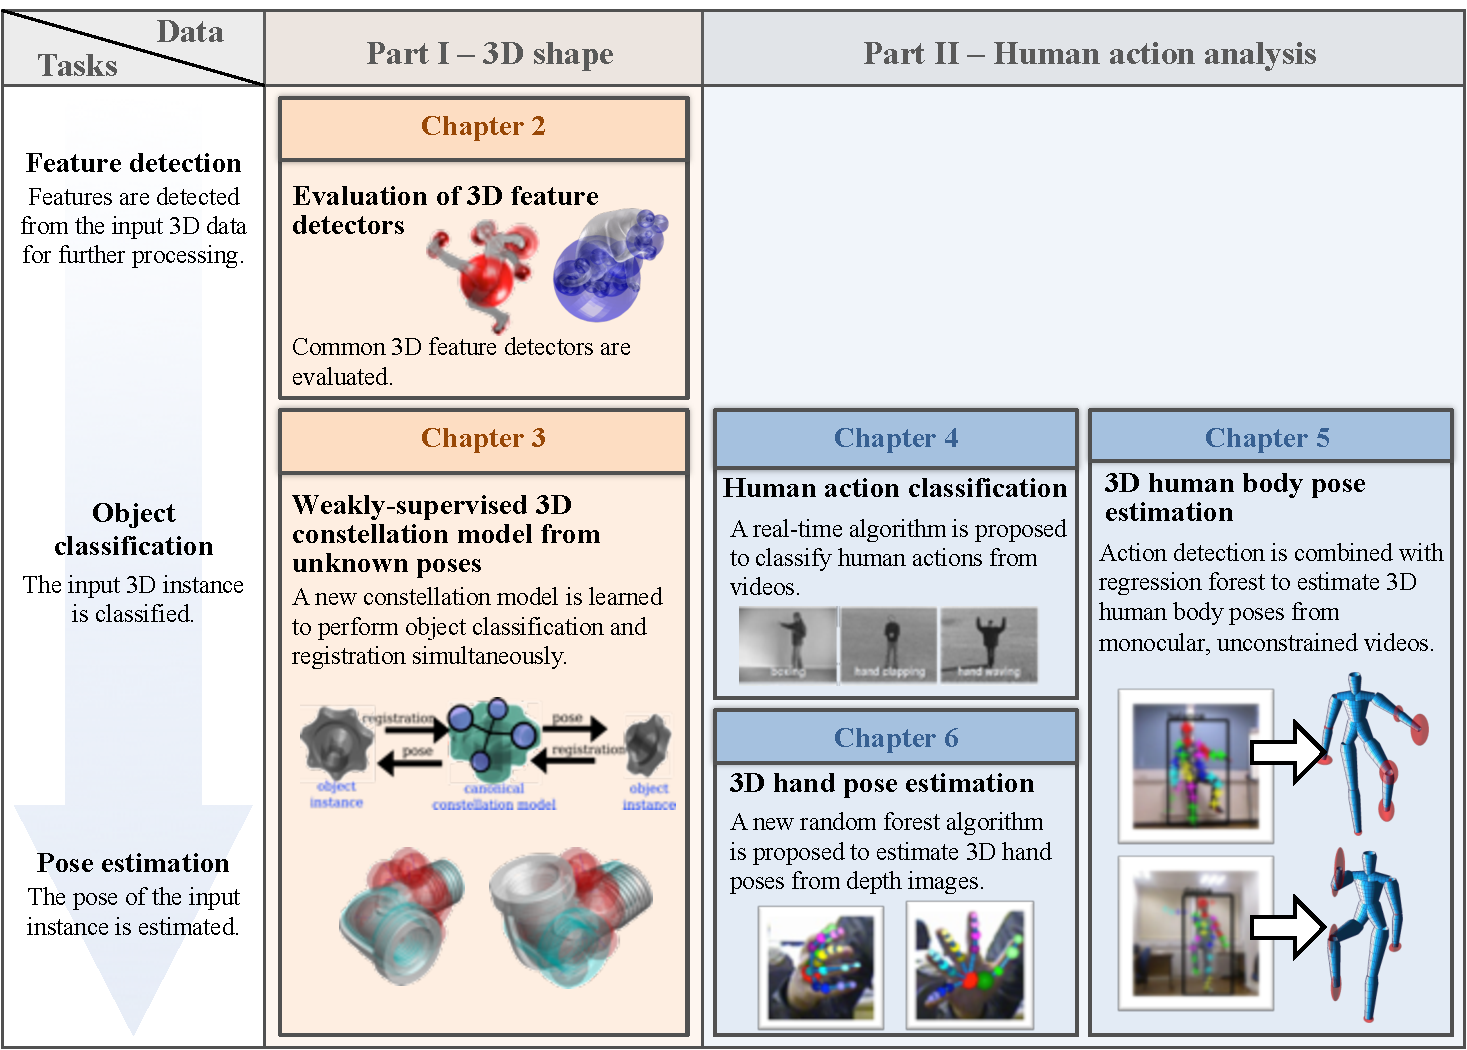
\includegraphics[width=1\linewidth]{./fig/intro/intro2.pdf}
\caption{\textbf{Thesis outline}. Part I is concerned with the feature detection, classification and pose estimation of 3D geometric shapes. Part II proposes new approaches to human action classification and pose estimation from spatiotemporal data.} 
\label{fig/intro/outline}
\end{figure}

\subsection{Limiting the scope}

% Some thing which is not considered?
In order to concentrate on the most important and relevant topics, several areas of 3D object recognition are not considered within this thesis. 

The first is recognition of textured 3D meshes \cite{Zaharescu2009, Bronstein2011, Kokkinos2012}. Textured meshes are a standard means of representing 3D shapes in computer graphics and computer-aided design (CAD) tasks. 
%However, realistic 3D shape data are usually captured in textureless point clouds, depth images or voxels. 
However, real world 3D objects are usually captured in the form of texture-less point clouds, depth images or voxels. 
In addition, instances of the same object class can have different textures. Whilst texture-based appearance features are still useful for instance recognition, they are not suitable for shape classification tasks.  

The second area is instance-based 3D object recognition, \eg \cite{Mian2006, Rothganger2006, Shang2010}. Such system is trained to recognise one specific object instance, rather than different object instances from the same class. Its performance of object recognition and pose estimation relies mainly on feature matching between the training exemplars and the testing instance. As a result, this approach cannot be generalised to 3D object classification and category-based pose estimation, which are the main topics of this thesis.    
   
% The performance of object recognition and pose estimation of such approach rely mainly on feature matching between the model and query object instance. 

Thirdly, marker-based motion capture systems are not included in the scope of this thesis. They have been widely employed in computer-generated imagery for films and games. Markers are localised easily from a calibrated camera system using multi-view geometry. Poses may then be estimated straightforwardly by mapping the markers to a predefined articulated skeleton. In this thesis, such a marker-based approach is not considered because it is restricted to carefully-controlled studio environments.  
% With a calibrated camera network, 3D human poses can be recovered using marker-based approaches easily.  
 
Finally, body shape estimation from images and videos are not considered in the thesis \cite{Guan2009, Rother2009, Chen2011}. 
Body shape estimation is concerned primarily with the accurate reconstruction of 3D human shapes, rather than the inference of parameterised poses of an articulated model. Conversely, body pose estimation is concerned with understanding the semantics of the subject and the scene, rather than reconstructing them accurately. 
%It reconstructs 3D human shapes directly from testing data, instead of parameterised poses of an articulated model. Body pose estimation is concerned with understanding the semantics of the subject and the scene, rather than reconstructing them accurately. 

\subsection{Outline}

The structure of this thesis is outlined in figure \ref{fig/intro/outline}. In part I, chapter \ref{chap/eval} and chapter \ref{chap/reg} focus on the recognition and pose estimation of 3D shapes; in part II, chapters \ref{chap/act}, \ref{chap/body} and \ref{chap/hand} focus on human action analysis, including action categorisation and 3D pose estimation of human body and hand gestures. Chapter \ref{chap/conclusion} concludes the thesis with possible directions for future research. 

\subsection*{Part I --- 3D Shape}

%\paragraph{Chapter 2.} This chapter presents a literature review of 3D shape processing techniques.  Recent topics about 3D feature detection, shape representation, shape recognition and pose estimation are discussed.  

\subsubsection*{Chapter 2. Evaluation of 3D feature detectors} 
\iffalse
A performance evaluation of volumetric 3D interest points is presented in this chapter. 
It first provides an overview of current volumetric interest point detectors found in the literature. 
A selection of interest point detectors are then evaluated quantiatively using a new performance metric. 
% Finally, the qualitative characteristics of each of the detectors is also discussed.
The qualitative characteristics of the interest points are compared and analysed.
(This work has also appeared in the International Journal of Computer Vision, volume 102 (1--3), 2013 \cite{Yu2013a}.)  
\fi

Feature detection is an essential steps for many 3D object recognition algorithms. Various 3D interest point detectors have been proposed for different applications. While there exist comprehensive reviews for 2D interest point detectors, \eg \cite{Mikolajczyk2004}, 3D interest points have not been studied extensively. 

A performance evaluation of volumetric 3D interest points is presented in this chapter. 
It first provides an overview of current volumetric interest point detectors found in the literature. 
A selection of interest point detectors are then evaluated quantiatively using the repeatability area score, which is a new unified metric that describes the repeatability and accuracy of an interest point detector. 
% Finally, the qualitative characteristics of each of the detectors is also discussed.
The qualitative characteristics of the interest points are compared.  
This chapter concludes by categorising and analysing the experimental results of the candidate detectors.
% ; it is suggested that the choice of 3D interest point detector is application depedent.

(This work has also appeared in the International Journal of Computer Vision, volume 102 (1--3), 2013 \cite{Yu2013a}.)  

\subsubsection*{Chapter 3. 3D Constellation model from unknown pose}

This chapter is concerned with the tasks of classification and pose estimation of 3D geometric shapes. 
Traditional part-based models, such as the constellation model \cite{Weber2000}, do not infer a complete object pose during testing. In addition, their training instances are required to be registered to a common reference frame.

A weakly-supervised constellation model for simultaneous 3D shape recognition and pose estimation is proposed. 
It learns the shape, appearance and pose of an object class from training exemplars, \eg images or point clouds, which contain examples of the object in unknown poses. 
A new particle-based expectation-maximisation (EM) algorithm is employed to learn the proposed constellation model. During the training process, data instances are registered by the proposed particle-based EM algorithm.
The proposed model also performs classification and registration simultaneously in testing. 

\subsection*{Part II --- Human action analysis}

%\paragraph{Chapter 5.} This chapter introduces various sub-problems in human action analysis, including human action recognition, body pose estimation and hand pose estimation.  It discusses the application of random forests and its variants to model human actions and poses. It also reviews the existing approaches for the above sub-problems. 

\subsubsection*{Chapter 4. Human action classification} 
\iffalse
This chapter addresses the recognition sub-problem in human action analysis. 
A spatiotemporal semantic and structural forest is proposed to recognise human actions in real-time.    
(This work has been presented in the 2010 British Machine Vision Conference \cite{Yu2010}.)  
\fi

This chapter addresses the sub-problem of human action classification. A real-time human action classification framework is proposed. Video patches are encoded to visual codewords efficiently by a semantic texton forest \cite{Shotton2008}. The Hierarchical Spatiotemporal Relationship Match (HSRM) is introduced to capture both appearance and structural information of the visual codewords. The classification result from the HSRM algorithm is combined with the output of a traditional bag-of-words model, using a late fusion scheme.  

(This work has been presented in the 2010 British Machine Vision Conference \cite{Yu2010}.)  

\subsubsection*{Chapter 5. 3D human body pose estimation} 
\iffalse
This chapter presents a new approach to 3D body pose estimation in unconstrained, monocular videos. 
A new hybrid decision forest is introduced, in order to perform action detection and pose estimation simultaneously. 
Pose estimation is based on action detection, which includes joint classification and localisation of actions in videos. 
(This work has been presented in the 2013 IEEE Conference on Computer Vision and Pattern Recognition \cite{Yu2013}.)  
% By combining regression random forests with action detection, the proposed method infers 3D poses from unconstrained, monocular videos. 
\fi

This chapter aims to develop a new approach to estimate 3D body poses from unconstrained, monocular videos. 
A deformable part model (DPM) is employed to detect 2D body parts, which are highly robust to appearance changes and cluttered backgrounds. 2D shape-based feature vectors are computed from the detected body parts for 3D pose estimation. 

Two different random forest algorithms are introduced to estimate 3D body pose from the 2D feature vectors. 
A new hybrid action detection forest is proposed to perform action detection and pose estimation. A regression forest is also presented to estimate 3D joint locations at the same time. Pose estimation results from the two forests are combined using a probabilistic late fusion scheme. A new Action-Pose-Estimation (APE) dataset is collected to evaluate the performances of action classification and pose estimation simultaneously. 

(This work has been presented in the 2013 IEEE Conference on Computer Vision and Pattern Recognition \cite{Yu2013}.)  

\subsubsection*{Chapter 6. 3D hand pose estimation} 

\iffalse
This chapter addresses the sub-problem of articulated hand pose estimation. The Semi-supervsed Transductive Regression forest (\STR\ forest) is proposed to estimate 3D hand poses from noisy depth images.
The action detection tree learning algorithm introduced in chapter \ref{chap/body} is extended to perform various tasks, including viewpoint classification, joint classification and regression. 
A data-driven inverse kinematic technique is proposed to refine the occluded joints. (This work has been presented in the 14th IEEE International Conference of Computer Vision, 2013 \cite{Tang2013}.)
\fi

This chapter addresses the sub-problem of articulated hand pose estimation.  Unlike body poses, hand poses are prone to self-occlusions and viewpoint changes. Realistic training data are costly via manual labelling, because of sampling noise and the complex structure of human hands. 

In this work, the Semi-supervised Transductive Regression forest (\STR\ forest) is proposed. Similar to the action detection forest in chapter \ref{chap/body}, the \STR\ forest performs various recognition tasks, including viewpoint classification, joint classiication and regression. It utilises both synthetic and realistic training data by transductive learning, which creates associations between the two training dataset. In addition, semi-supervised learning is employed in the \STR\ forest training algorithm, in order to utilise the unlabelled data.
Furthermore, a data-driven inverse kinematic technique is also presented to recover the occluded joints from the \STR\ forest.

(This work has been presented in the 14th IEEE International Conference of Computer Vision, 2013 \cite{Tang2013}.)
